\documentclass[]{article}
\usepackage{amsmath,amssymb,amsfonts,amsbsy}
\usepackage{indentfirst}
\usepackage{fancybox}
\usepackage{graphicx}
\usepackage{soul,soulutf8}
\usepackage{url,color}
\usepackage{fullpage}
\usepackage{tikz}
\usepackage{float}
\usepackage{subcaption}
\usepackage{url}
\usepackage{wrapfig}
\usepackage{xcolor}
\usepackage{listings}

\usetikzlibrary{positioning}
\usetikzlibrary{shapes, arrows}
\usetikzlibrary{decorations.pathreplacing}

\lstset{
	basicstyle=\footnotesize\ttfamily,
	commentstyle=\color{red},
	keywordstyle=\color{blue}
}

\usepackage[autocite=footnote,
    backend=bibtex,
    citestyle=ieee,
    isbn=false,
    doi=false,
    url=false
]{biblatex}
\addbibresource{IT.bib}


%\baselineskip=15pt
% \pagestyle{plain}   %with page numbers
% \pagestyle{empty} %without page numbers

\renewcommand{\baselinestretch}{1.25}
\newcommand{\R}{\mathbb{R}}
\newcommand{\cX}{\mathcal{X}}
%\newcommand{\tr}{\mathrm{tr}}
\renewcommand{\st}{\mathrm{s.t.}}

% Define block styles
\tikzstyle{decision} = [diamond, draw, fill=blue!20, 
text width=4.5em, text badly centered, node distance=3cm, inner sep=0pt]
\tikzstyle{block} = [rectangle, draw, fill=blue!20, 
text width=6em, text centered, rounded corners, minimum height=4em, minimum width=8em, scale=.6]

\tikzstyle{blockq} = [rectangle, draw, fill=red!20, 
text width=6em, text centered, rounded corners, minimum height=4em, minimum width=8em, scale=.6]

\tikzstyle{line} = [draw, -latex']
\tikzstyle{cloud} = [draw, ellipse,fill=red!20, node distance=3cm,
minimum height=2em]

\definecolor{darkgreen}{HTML}{006622}

%\usepackage[toc]{multitoc}\begin{minipage}{.6\textwidth}

\begin{document}

%Enter your title here
\title{Profile-Guided Source Coding in Dual-Compilation}
%Enter your name Here
\author{Chenhao Wu}
\date{May, 2019}

\makeatletter
\let\inserttitle\@title
\let\insertauthor\@author
\makeatother

\begin{titlepage}
\centering
{   \textsc{\Large CIE 6020 (Spring, 2018)}\\[0.5 cm]}
{\Large\bf Report: \inserttitle}\\[.2in]
Name: \underline{\quad\quad \insertauthor \quad\quad  
}
\hspace{0.3in}
ID Number: \underline{\quad\quad
%Enter Your ID number Here
117010285
\quad\quad}
\vspace{0.5 cm}\\
\fbox{\parbox{\textwidth}{
\begin{itemize}
% \item 
% Date assigned: Friday 19/1/2018
% \item 
% Date due: Thursday 1/2/2018, 11:55 PM
\item
This cover sheet must be signed and submitted along with the report on additional sheets
\item
By submitting this report with my name affixed above,
\begin{itemize}
%\item
%I understand that report submitted at 11:56 PM or later will not be accepted,
\item
I acknowledge that I am aware of the University policy concerning academic misconduct (appended below),
\item
I attest that the work I am submitting for this assignment is solely my own, and
\item
I understand that suspiciously similar homework submitted by multiple
individuals will be reported to School and Registry for investigation.
\end{itemize}
\item
Academic Misconduct in any form is in violation of CUHK(SZ)'s Student Disciplinary Regulations and will not be tolerated. This includes, but is not limited to: copying or sharing answers on tests or assignments, plagiarism, having someone else do your academic work or working with someone on homework when not permitted to do so by the instructor. Depending on the act, a student could receive an F grade on the test/assignment, F grade for the course, and could be suspended or expelled from the University.
\end{itemize}}}
\end{titlepage}

%%% Begin of the report 
\maketitle

%\begin{abstract}
%Within this decade, the computing performance of mobiles and embedded systems have been significantly raised such that more computing workloads can be undertaken on mobiles and embedded systems, such as digital image processing, augmented-reality applications, and so on. In practice, one of the critical bottlenecks in mobiles and embedded systems design and optimization is the run-time memory space and power consumption. Since the complexity of program and data set grew much faster than the performance of memory capacity in the mobile and embedded system, rather than merely use expensive computing components to feed the needs of applications with high computing overhead, it is more promising to find ways to best utilize the system use of memory space. To realize this objective, we proposed a profile-guided source coding (PGSC), which will perform an adaptive compiler-guided data compression on memory space during run-time according to different applications and run-time environment.
%\end{abstract}

\section{Introduction}
Within this decade, the computing performance of mobiles and embedded systems have been significantly raised such that more computing workloads can be undertaken on mobiles and embedded systems, such as digital image processing, machine learning and deep learning applications, augmented-reality applications, and so on. In practice, one of the critical bottlenecks in mobiles and embedded systems design and optimization is the run-time memory space and power consumption. Since the complexity of program and data set grew much faster than the performance of memory capacity in the mobile and embedded system, rather than merely use expensive computing components to feed the needs of applications with high computing overhead, it is more promising to find ways to best utilize the system use of memory space. To realize this objective, we proposed a profile-guided source coding (PGSC), which will perform an adaptive compiler-guided data compression on memory space during run-time according to different applications and run-time environment. \par 

%figure 1, 2, 3
\begin{figure}[H]
\begin{minipage}[b][8cm][s]{.27\textwidth}
	\centering
	\vfill
	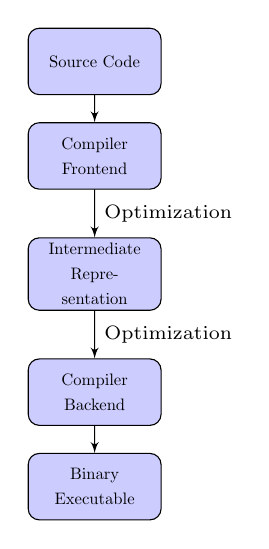
\begin{tikzpicture}[node distance = 2cm, auto]
	
	% Place nodes
	\node [block] 								(Source Code) 					{Source Code};
	\node [block, below of=Source Code] 		(Compiler Frontend)  			{Compiler Frontend};
	\node [block, below of=Compiler Frontend, yshift=-0.5cm] (IR)				{Intermediate Representation};
	\node [block, below of=IR, yshift=-0.5cm]	(Compiler Backend)				{Compiler Backend};
	\node [block, below of=Compiler Backend]	(Binary Executable)				{Binary Executable};
	
	%Draw edges
	\path [line] (Source Code) 		    -- 										(Compiler Frontend);
	\path [line] (Compiler Frontend)    -- node {\scriptsize Optimization} 		(IR);
	\path [line] (IR) 					-- node {\scriptsize Optimization} 		(Compiler Backend);
	\path [line] (Compiler Backend)		--										(Binary Executable);
	
	\end{tikzpicture}
	
	\vfill
	\captionsetup{justification=centering}
	\caption{Traditional Compilation Procedure}
	\label{fig:compil}
	
	\vspace{\baselineskip}
\end{minipage}\qquad
\begin{minipage}[b][8cm][s]{.35\textwidth}
	\centering
	\vfill
	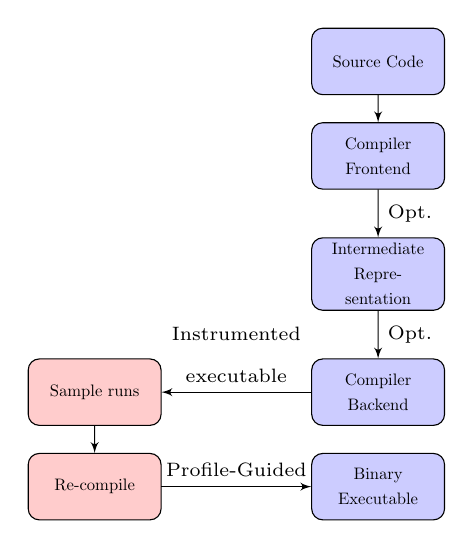
\begin{tikzpicture}[node distance = 2cm, auto]
	
	% Place nodes
	\node [block] 								(Source Code) 					{Source Code};
	\node [block, below of=Source Code] 		(Compiler Frontend)  			{Compiler Frontend};
	\node [block, below of=Compiler Frontend, yshift=-0.5cm] (IR)				{Intermediate Representation};
	\node [block, below of=IR, yshift=-0.5cm]	(Compiler Backend)				{Compiler Backend};
	\node [block, below of=Compiler Backend]	(Binary Executable)				{Binary Executable};
	\node [blockq, left of=Compiler Backend, xshift=-4cm] (SR)				{Sample runs};
	\node [blockq, left of=Binary Executable, xshift=-4cm] (Re-Compile)		{Re-compile};
	
	%Draw edges
	\path [line] (Source Code) 		    -- 										(Compiler Frontend);
	\path [line] (Compiler Frontend)    -- node {\scriptsize Opt.} 		(IR);
	\path [line] (IR) 					-- node {\scriptsize Opt.} 		(Compiler Backend);
	\path [line] (Compiler Backend)		-- node[above, align=center] {\scriptsize Instrumented\\ \scriptsize executable} (SR);
	\path [line] (SR)					-- 									    (Re-Compile);
	\path [line] (Re-Compile)			-- node {\scriptsize Profile-Guided}	(Binary Executable);
	
	\end{tikzpicture}
	\vfill
	\captionsetup{justification=centering}
	\caption{Compilation Procedure with PGO}
	\label{fig:compilpgo}
\end{minipage}\qquad
\begin{minipage}[b][8cm][s]{.3\textwidth}
	\centering
	\vfill
	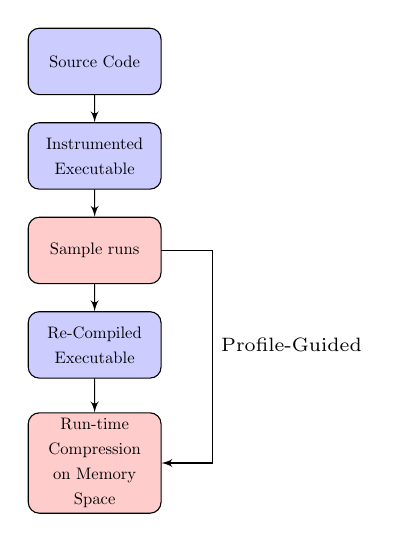
\begin{tikzpicture}[node distance = 2cm, auto]
	
	% Place nodes
	\node [block] 								(Source Code) 					{Source Code};
	\node [block, below of=Source Code] 		(IE) 					 		{Instrumented Executable};
	\node [blockq, below of=IE] 				(SR)							{Sample runs};
	\node [block, below of=SR] 					(Re-Compiled Executable)		{Re-Compiled Executable};
	\node [blockq, below of=Re-Compiled Executable, yshift=-0.5cm] (RC)							{Run-time Compression on Memory Space};	
	\node [label, right of=Re-Compiled Executable, xshift=0.5cm]								(PF)							{\scriptsize Profile-Guided};
	
	%Draw edges
	\path [line] (Source Code) 		    -- 										(IE);
	\path [line] (IE) 					-- 										(SR);
	\path [line] (SR)					--									 	(Re-Compiled Executable);
	\path [line] (Re-Compiled Executable) --									(RC);
	\path [line] (SR)					--++ (1.5, 0)  |-						(RC);
	
	\end{tikzpicture}
	\vfill
	\caption{Profile-Guided Source Coding}
	\captionsetup{justification=centering}
	\label{fig:compilpgosrc}
\end{minipage}
\end{figure}

The idea of this approach comes from a modern compilation technique, Profiled-Guided Optimization (PGO), that as shown in Figure 1 and Figure 2, differed from the traditional approach \cite{CompilerDesign}, the compiler will perform a recompilation based on initial executable and sample runs. A profile, for instance, breaks the source code into blocks and devises a table of the frequency each block is executed via sample runs, and during recompilation, code blocks will be reordered with respect to the frequency table. For example, blocks with higher frequency will be allocated in memory area with lower memory address and blocks with lower frequency will be allocated in higher address so that the additional I/O overhead consumed in function callbacks will be reduced. Similar to previous compiler optimization methods, like the deletion of unreachable code, the constant folding optimization and propagation optimization, the objective of PGO is to further reduce the redundancy of unnecessary and/or unimportant logic branches in the source program. \par 
The usage of this approach, however, can be extended into attempts in reducing the memory space, that after sample runs, not only the frequency of code blocks can be collected, but also the preliminary investigation of frequency that each block of memory is accessed can be gathered as well. As shown in Figure 3, the procedure of PGSC consists of a dual-stage compilation, that the compiler will initially compile the source code into an instrumented executable, and based on a profile generated after sample runs, the compiler will re-compile the source code such that during the run-time, the program will compress specific areas of memory space in order to reduce the redundancy of memory use, and will instantaneously decompress the compressed contents whenever the program needs. \par 
In the tide that more and more applications on mobile and embedded systems behave to buffer long arrays of audio, images and video frames into the memory space during run-time, that in a low frequency the program access to them but they still need to be remained in the memory space, for usages like intermediate training matrices, sample sets of images and so on, PGSC can regularly compress them to reduce the buffer size. The compression is compiler-guided, thus it can be performed no matter which optimization has been applied onto the program and what third-party libraries the program has imported. \par 
In this report we will briefly introduce the control flow of PGSC, the methodologies we applied to perform the compression over memory space, and the implementation of a compiler with PGSC. 

\section{Related Work}
One solid work to use data compression for run-time memory system utilization had been practiced by Ozcan Ozturk, Mahmut Kandemir and Mary Jane Irwin \cite{OO2009}, in which they designed a computational algorithms to compress the run-time data. Compiler-guided compression are also considered in compiler optimization related work \cite{MSAli2008}\cite{KSKO2017}\cite{MTK2011}. In software engineering, a profile-directed feedback was firstly applied in IBM kernel compilation \cite{IBM}, and also adopted in the build of Firefox and Chromium \cite{firefox}\cite{Chrome}. Previous work using profile-guided compiler optimization had proved that this method of optimization is able to reduce the average memory occupancy from 15\% to 50\%. 
	
\section{Implementation}

	\subsection{Structural RAM Assignment for Run-time Compression}
	In a run-time environment with the stack-allocation strategy, a consecutive memory area will be divided into segments, and allocated by activation records and run-time objects. The order of allocation is arbitrary, and therefore in a while after the program being run, the allocated areas and free areas are interlaced. The system manages and looks up an allocation table to free up allocated space and reuse freed space. \par 
	As shown in Figure 5, an activity record consists of a sequence of run-time data and pointers towards the control \& access links. \par 
	% figure 4, 5
	\begin{figure}[H]	
	\begin{minipage}[b][4.5cm][s]{.5\textwidth}
		\centering
		\vfill
		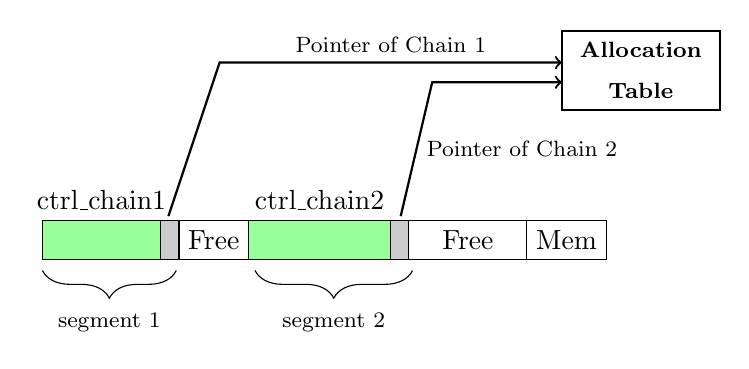
\begin{tikzpicture}
			\node[draw, fill=green!40, minimum width=15mm, minimum height=5mm, label=above:ctrl\_chain1] (almem1) {};
			\node[draw, fill=gray!40, minimum width=2mm, minimum height=5mm, right=-\pgflinewidth of almem1,,](p1) {};
			\node[draw, minimum width=8mm, minimum height=5mm, right=-\pgflinewidth of p1,,](om1) {Free};
			\node[draw, fill=green!40, minimum width=18mm, minimum height=5mm, right=-\pgflinewidth of om1,, label=above:ctrl\_chain2] (almem2) {};
			\node[draw, fill=gray!40, minimum width=2mm, minimum height=5mm, right=-\pgflinewidth of almem2](p2) {};
			\node[draw, minimum width=15mm, minimum height=5mm, right=-\pgflinewidth of p2,,](om2) {Free};
			\node[draw, minimum width=3mm, minimum height=5mm, right=-\pgflinewidth of om2,,] (M) {Mem};
			
			\draw [decorate,decoration={brace,amplitude=10pt,mirror,raise=4pt},yshift=0pt]
				  (-0.75,-0.25) -- (0.95, -0.25) node [black,midway,yshift=-0.8cm] {\footnotesize segment 1};
			\draw [decorate,decoration={brace,amplitude=10pt,mirror,raise=4pt},yshift=0pt]
			(1.95,-0.25) -- (3.95, -0.25) node [black,midway,yshift=-0.8cm] {\footnotesize segment 2};
			
			\draw [black, thick, ->] (0.85, 0.3) -- (1.5, 2.25) -- node [midway, align=center, above] {\footnotesize Pointer of Chain 1}(5.85, 2.25);
			\draw [black, thick, ->] (3.8, 0.3) -- node [midway, align=left, right] {\footnotesize Pointer of Chain 2} (4.2, 2) -- (5.85, 2);
			
			\node[draw, minimum width=20mm, minimum height = 10mm, line width=0.25mm, align=center] at (6.85, 2.15) (memory map) {\footnotesize \textbf{Allocation} \\ \footnotesize \textbf{Table}};
			
		\end{tikzpicture}	
		\vfill
		\captionsetup{justification=centering}
		\caption{Memory Allocation}
		\label{fig:memaloc}	
		\vspace{\baselineskip}
	\end{minipage} \qquad
	\begin{minipage}[b][8cm][s]{.5\textwidth}
		\centering
		\vfill
		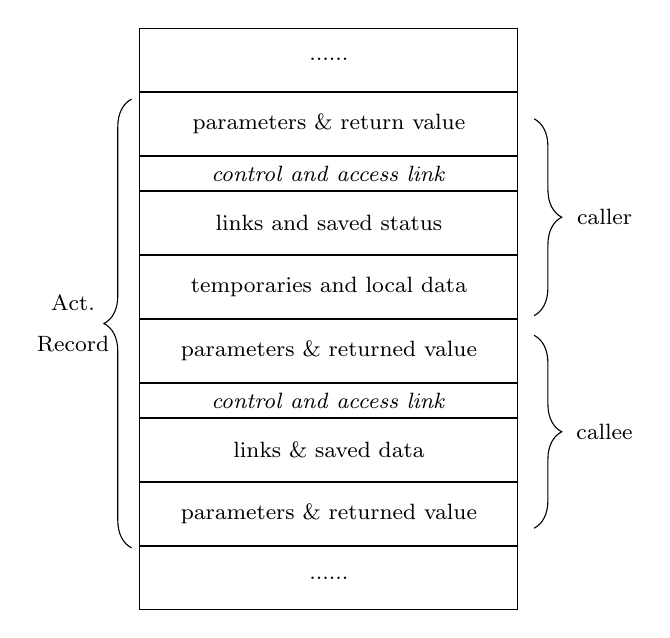
\begin{tikzpicture}
			\node[draw, minimum width=48mm, minimum height=8mm] (om1) {\footnotesize ......};
			\node[draw, minimum width=48mm, minimum height=8mm, below=0mm of om1] (s1) {\footnotesize parameters \& return value};
			\node[draw, minimum width=48mm, minimum height=4mm, below=0mm of s1] (s0) {\footnotesize \textit{control and access link}};
			\node[draw, minimum width=48mm, minimum height=8mm, below=0mm of s0]  (s2) {\footnotesize links and saved status};
			\node[draw, minimum width=48mm, minimum height=8mm, below=0mm of s2]  (s3) {\footnotesize temporaries and local data};
			\node[draw, minimum width=48mm, minimum height=8mm, below=0mm of s3]  (s4) {\footnotesize parameters \& returned value};
			\node[draw, minimum width=48mm, minimum height=4mm, below=0mm of s4]  (s5) {\footnotesize \textit{control and access link}};
			\node[draw, minimum width=48mm, minimum height=8mm, below=0mm of s5]  (s6) {\footnotesize links \& saved data};
			\node[draw, minimum width=48mm, minimum height=8mm, below=0mm of s6]  (s7) {\footnotesize parameters \& returned value};
			\node[draw, minimum width=48mm, minimum height=8mm, below=0mm of s7]  (s8) {\footnotesize ......};
			
			\draw[decorate,decoration={brace,amplitude=10pt,mirror,raise=3pt},yshift=0pt,align=center] (-2.4, -0.5) -- (-2.4, -6.2) node[black,midway,xshift=-0.85cm] {\footnotesize Act.\\ \footnotesize Record};	
			\draw[decorate,decoration={brace,amplitude=10pt,raise=3pt},yshift=0pt] (2.5, -0.75) -- (2.5, -3.25) node[black,midway,xshift=1cm] {\footnotesize caller};
			\draw[decorate,decoration={brace,amplitude=10pt,raise=3pt},yshift=0pt] (2.5, -3.5) -- (2.5, -5.95) node[black,midway,xshift=1cm] {\footnotesize callee};
			
		\end{tikzpicture}
		\vfill
		\captionsetup{justification=centering}
		\caption{Task Stack}
		\label{fig:taskstack}	
		\vspace{\baselineskip}
	\end{minipage}


	\end{figure}
	Our scheme to achieve data compression on RAM requires a sufficient analysis on run-time memory access records, and then we will separate the entire memory space into two elementary areas, run-time area and compressed area. Kindly note that the separation of memory space is not an actual separation on memory sequence, but applying two different tables to manage respective memory space. \par 
	\begin{figure}[H]
		\centering
		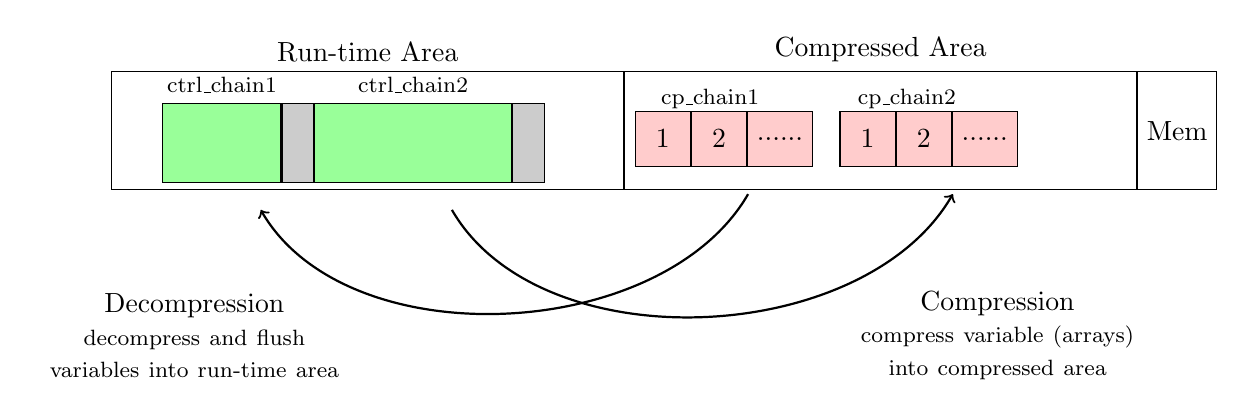
\begin{tikzpicture}[line/.style={->,shorten >=0.4cm,shorten <=0.4cm}]
			\node[draw, minimum width=65mm, minimum height=15mm, align=center, label=above:Run-time Area] at (0, 0) (run-time) {};
			\node[draw, minimum width=65mm, minimum height=15mm, align=center, right=0mm of run-time, label=above:Compressed Area] (compressed) {};
			\node[draw, minimum width=10mm, minimum height=15mm, align=center, right=0mm of compressed] (memory) {Mem};
			
			\node[draw, fill=green!40, minimum width=15mm, minimum height=10mm, align=center, label={[above, font=\footnotesize, align=center]ctrl\_chain1}] at (-1.85, -0.15) (rt1) {};
			\node[draw, fill=gray!40, minimum width=4mm, minimum height=10mm, align=center, right=0mm of rt1] (pt1) {};
			\node[draw, fill=green!40, minimum width=25mm, minimum height=10mm, align=center, label={[above, font=\footnotesize, align=center]ctrl\_chain2}, right=0mm of pt1] (rt2){};
			\node[draw, fill=gray!40, minimum width=4mm, minimum height=10mm, align=center, right=0mm of rt2] (pt2) {};
			
			\node[draw, fill=red!20, minimum width=7mm, minimum height=7mm, align=center] at (3.75, -0.1) (r11) {1};
			\node[draw, fill=red!20, minimum width=7mm, minimum height=7mm, align=center, right=0mm of r11] (r12) {2};
			\node[draw, fill=red!20, minimum width=8mm, minimum height=7mm, align=center, right=0mm of r12] (rd) {......};
			\node[align=center] at (4.35, 0.4) (lr1) {\footnotesize cp\_chain1};
			
			\node[draw, fill=red!20, minimum width=7mm, minimum height=7mm, align=center] at (6.35, -0.1) (r21) {1};
			\node[draw, fill=red!20, minimum width=7mm, minimum height=7mm, align=center, right=0mm of r21] (r22) {2};
			\node[draw, fill=red!20, minimum width=8mm, minimum height=7mm, align=center, right=0mm of r22] (rd2) {......};
			\node[align=center] at (6.85, 0.4) (lr2) {\footnotesize cp\_chain2};
			
			\path [black, line, thick, out=-60,in=-120] (rt2) edge (rd2);
			\path [black, line, thick, out=-120,in=-60] (rd) edge (rt1);
			
			\node[align=center, text width=3.5cm] at (8, -2.6) 		(p1) {Compression \\ \baselineskip=10pt\footnotesize compress variable (arrays) into compressed area\par};
			\node[align=center, text width=4cm] at (-2.2,  -2.6)   (p2) {Decompression\\\baselineskip=1pt \footnotesize decompress and flush variables into run-time area\par};
			
			%\draw (pt1) to [out=-60, in=-120] (rd);
			
		\end{tikzpicture}
		\captionsetup{justification=centering}
		\caption{Run-time Compression \& Decompression}
		\label{fig:rtcd}
	\end{figure}
	In the compilation, the compiler specifies which areas of data need to be compressed during idle time, and also generate codeword of each segment, so as during run-time the program would automatically compress them from the run-time area into the compressed area. Whenever the compressed data are needed or being called, the program will instantaneously decompress the data from the compressed area, and flush them into the run-time buffer. The configuration of the compression is guided by the profile generated by sample runs, and also an initial compiling parameter \textit{-DEG\_COMP}, which represents the degree of compression. For instance, if the constraint of the system memory is not strict, the degree of compression can then be tuned down in order to reduce the compression area and increase computing efficiency.\par  
	
	\subsection{Implementation of Run-time Compression Compiler}
	In this project, we applied a program profiler \textit{valgrind} and a widely used compiler framework \textit{LLVM} to implement the run-time compression compiler. For the first tool we used in the project, \textit{valgrind}, it has several internal tools to examine and track the record of allocation/free instructions called by the program on heap during run-time, including the information of how much heap memory the programs used and statistics of how much time the program access to each segment of allocated space. Also, it can also generate readable profiles after analysis, describing the behavior of the program and passing to consecutive process. \par 
	A sample profile used in our project is like following
	\begin{lstlisting}[language=bash, caption=(Sample Profile)]
$ cat ./sample_prof
desc: --time-unit=B --detailed-freq=1
cmd: ./sample1
time_unit: B
#-----------
snapshot=0
#-----------
time=0
mem_heap_B=0
mem_heap_extra_B=0
mem_stacks_B=0
heap_tree=detailed
n0: 0 (heap allocation functions) malloc/new/new[], --alloc-fns, etc.
#-----------
snapshot=1
#-----------
time=1016
mem_heap_B=1000
mem_heap_extra_B=16
mem_stacks_B=0
heap_tree=detailed
n1: 1000 (heap allocation functions) malloc/new/new[], --alloc-fns, etc.
n0: 1000 0x108730: main (in /home/vitowu/Github/CIE6020-CourseProj/test/valgrind_massif/sample1)
...
#-----------
snapshot=24
#-----------
time=30344
mem_heap_B=10000
mem_heap_extra_B=24
mem_stacks_B=0
heap_tree=detailed
n3: 10000 (heap allocation functions) malloc/new/new[], --alloc-fns, etc.
n2: 8000 0x1086FC: g (in /home/vitowu/Github/CIE6020-CourseProj/test/valgrind_massif/sample1)
n1: 4000 0x108712: f (in /home/vitowu/Github/CIE6020-CourseProj/test/valgrind_massif/sample1)
n0: 4000 0x10874C: main (in /home/vitowu/Github/CIE6020-CourseProj/test/valgrind_massif/sample1)
n0: 4000 0x108751: main (in /home/vitowu/Github/CIE6020-CourseProj/test/valgrind_massif/sample1)
n1: 2000 0x10870D: f (in /home/vitowu/Github/CIE6020-CourseProj/test/valgrind_massif/sample1)
n0: 2000 0x10874C: main (in /home/vitowu/Github/CIE6020-CourseProj/test/valgrind_massif/sample1)
n0: 0 in 1 place, below massif's threshold (1.00%)

==8260== ======== SUMMARY STATISTICS ========
==8260== 
==8260== guest_insns:  2,268,254
==8260== 
==8260== max_live:     73,104 in 2 blocks
==8260== 
==8260== tot_alloc:    73,104 in 2 blocks
==8260== 
==8260== insns per allocated byte: 31
==8260== 
==8260== 
==8260== ======== ORDERED BY decreasing "max-bytes-live": top 10 allocators ========
==8260== 
==8260== -------------------- 1 of 10 --------------------
==8260== max-live:    72,704 in 1 blocks
==8260== tot-alloc:   72,704 in 1 blocks (avg size 72704.00)
==8260== deaths:      1, at avg age 118,908 (5.24% of prog lifetime)
==8260== acc-ratios:  0.00 rd, 0.00 wr  (0 b-read, 16 b-written)
==8260==    at 0x4C29F9F: malloc (vg_replace_malloc.c:299)
==8260==    by 0x4EBA9BF: ??? (in /usr/lib/x86_64-linux-gnu/libstdc++.so.6.0.22)
==8260==    by 0x400F799: call_init.part.0 (dl-init.c:72)
==8260==    by 0x400F8AA: _dl_init (dl-init.c:30)
==8260==    by 0x4000C59: ??? (in /lib/x86_64-linux-gnu/ld-2.24.so)
==8260== 
==8260== -------------------- 2 of 10 --------------------
==8260== max-live:    400 in 1 blocks
==8260== tot-alloc:   400 in 1 blocks (avg size 400.00)
==8260== deaths:      none (none of these blocks were freed)
==8260== acc-ratios:  0.50 rd, 1.54 wr  (200 b-read, 616 b-written)
==8260==    at 0x4C2AD2F: operator new[](unsigned long) (vg_replace_malloc.c:423)
==8260==    by 0x108884: main (in /home/vitowu/Github/CIE6020-CourseProj/test/valgrind_dhat/sample2/prog)
==8260== 
==8260== Aggregated access counts by offset:
==8260== 
==8260== [   0]  3 3 3 3 3 3 3 3 3 3 3 3 3 3 3 3 
==8260== [  16]  4 4 4 4 4 4 4 4 4 4 4 4 4 4 4 4 
==8260== [  32]  3 3 3 3 3 3 3 3 3 3 3 3 3 3 3 3 
==8260== [  48]  3 3 3 3 3 3 3 3 3 3 3 3 3 3 3 3 
==8260== [  64]  3 3 3 3 3 3 3 3 3 3 3 3 3 3 3 3 
==8260== [  80]  3 3 3 3 3 3 3 3 3 3 3 3 3 3 3 3 
==8260== [  96]  3 3 3 3 3 3 3 3 3 3 3 3 3 3 3 3 
==8260== [ 112]  3 3 3 3 3 3 3 3 3 3 3 3 3 3 3 3 
==8260== [ 128]  3 3 3 3 3 3 3 3 3 3 3 3 3 3 3 3 
==8260== [ 144]  3 3 3 3 3 3 3 3 3 3 3 3 3 3 3 3 
==8260== [ 160]  3 3 3 3 3 3 3 3 3 3 3 3 3 3 3 3 
==8260== [ 176]  3 3 3 3 3 3 3 3 3 3 3 3 3 3 3 3 
==8260== [ 192]  3 3 3 3 3 3 3 3 1 1 1 1 1 1 1 1 
==8260== [ 208]  1 1 1 1 1 1 1 1 1 1 1 1 1 1 1 1 
==8260== [ 224]  1 1 1 1 1 1 1 1 1 1 1 1 1 1 1 1 
==8260== 
==8260== ==============================================================

	\end{lstlisting}
	from which we can obtain the analysis of allocate/free and read/write instructions on RAM. \par 
	The second tool, \textit{LLVM}, stands for a flexible compiler framework with great extensibility, allowing researchers in the area of compiler optimization to easily load their own customized optimization modules into compilation process and control the ordering of compilation. In  this project, we implement three \textit{LLVM opt} module, which are \textbf{\textit{ProfileManager.so}}, the agent to parse profiles; \textbf{\textit{Compression.so}}, the module to emit compression/decompression functions into original program; and \textbf{\textit{LZO.so}}, a library to provide compression and decompression methods to the optimizer. \par 
	The primary compression method we applied in the project is Lempel–Ziv–Oberhumer compression, During the second compilation, \textit{LLVM} will substitute part of reading/writing instructions with function calls of LZO compressing/decompressing according to the profile. Eventually, for writing instructions of some data structure being allocated in run-time, the finalized program does not directly write the raw data onto the RAM, and instead, the program compress them and write the compressed data into compressed area. And also, the reading instructions are being substituted by decompression functions in a similar approach. \par 
	\subsection{Work Flow}
	An simplified work-flow of Run-time Compression Compiler is as following:
	\begin{enumerate}
		\item \textit{LLVM} guides clang/clang++ (generic raw compilation) to initially compile the source code into binary
		\item Insert \textit{valgrind} into the binary program and run for an arbitrary long period, profiling the program on heap usage
		\item Passing the profile to \textit{LLVM} and substitute read/write instructions according to profile
	\end{enumerate} 
	
\section{Experiments}
	\subsection{Testing Programs}
	To examine the performance of run-time compiler, we apply several testing programs to make comparison between ordinary compiler and compiler with profiled-guided source coding. 
	\begin{table}[H]
		\begin{tabular}{|l|l|}
	        \hline
	        Testing program & Functionality \\ \hline 
			LU-Decomposition                      & Solve a set of linear equations using LU decomposition        \\ \hline
			Facial Recognition                    & Capture and learn new faces from camera                       \\ \hline
			LZ Compression                        & Tool to compress literature text using LZO                    \\ \hline
			Huffman Coding                        & Tool to compress literature text using Huffman coding on word \\ \hline
		\end{tabular}
	\end{table}
	
	\subsection{Testing Environment}
	\begin{itemize}
		\item \textbf{Operating System}: Debian 9 Virtual Machine
		\item \textbf{Architecture}: x86-64
		\item \textbf{RAM}: 512 MB
		\item \textbf{Number of Processors}: 1 
		\item \textbf{Clock Frequency} 2.8 GHz
		\item \textbf{Generic Compiler}: clang/clang++
	\end{itemize}
	The number of processors and RAM size were intended to be limited in order to simulate a similar environment as on mobile phones and embedded systems, in which CPU and RAM overhead are much more significant than personal computers.

\section{Result}
	In the experiment section, we compiled the testing programs by two different approaches. The first approach is using \textit{clang} to compile the source code without adding any optimization flag. The second approach is using Run-time Compression Compiler to compile the testing programs, which is implemented in this project. We analyzed the maximum memory occupancy, the average memory occupancy, and extra time in compilation respectively, and summarize to a comparison between this two approaches as following
	\begin{table}[H]
		\begin{tabular}{|l|l|l|l|l|l|}
			\hline
			Testing program    & MMO(clang) & AMO(clang) & MMO(RCC) & AMO(RCC) & Extra Time(RCC) \\ \hline
			LU-Decomposition   & 214.3 Mb   & 165.7 Mb   & 153.7 Mb & 53.9 Mb  & +47\%           \\ \hline
			Facial Recognition & 470.0 Mb   & 365.2 Mb   & 190.7 Mb & 80.3 Mb  & +239\%          \\ \hline
			LZ Compression     & 253.7 Mb   & 103.8 Mb   & 217.8 Mb & 93.7 Mb  & +65\%           \\ \hline
			Huffman Coding     & 324.1 Mb   & 214.7 Mb   & 293.7 Mb & 196.5 Mb & +53\%           \\ \hline
		\end{tabular}
	\end{table}
	where MMO stands for Maximum Memory Occupancy and AMO stands for Average Memory Occupancy. \par 
	From the result of experiments, we can find that by using run-time compression compiler, both the maximum memory occupancy and the average memory occupancy decreased. For LU-Decomposition and Facial Recognition programs, the decrease rate is than larger than the rest two programs, since during run-time, the former two programs would store lots of intermediate matrix and intermediate pictures array, which has much more redundancy than the latter two programs and then contribute to a higher compression rate. \par    
	Also, even though the extra compression time increased after applied run-time compression compiler, it is still within an acceptable range. Hence, for the most of applications in ordinary scenarios, applying run-time compression on them is useful and considerable.
	
\section{Conclusion and Future Work}
	In this report, we introduced our approach, as a compiler optimization, to delimit the memory occupancy. In our approach, we propose to use a profile-guided strategy and to apply source coding on RAM during run-time. Also, we implemented a run-time compression compiler and designed experiments to test and validate our approach. From the result we can conclude that, our approach is feasible in utilizing the memory occupancy with a considerable optimizing rate. One shortcoming occurred in the experiment is that the programs using run-time compression run slower than ordinary programs, since CPU has to distribute some computing resources to compress and decompress the data instantly. We believe that this problem is significant due to our approach is left in software-level optimization, and it would be reduced or even eliminated by using hardware-based compression. In the future, we would like to apply the technique illustrated in the report on hardware and compare the performance of them.
\printbibliography


\end{document}
